%
% aes.tex -- Beschreibung des AES Algorithmus
%
% (c) 2020 Prof Dr Andreas Müller, Hochschule Rapperswil
%
\section{Advanced Encryption Standard -- AES
\label{buch:section:aes}}
\rhead{Advanced Encryption Standard}
Eine wichtige Forderung bei der Konzeption des damals neuen
Advanced Encryption Standard war, dass darin keine ``willkürlich''
erscheinenden Operationen geben darf, bei denen der Verdacht
entstehen könnte, dass sich dahinter noch offengelegtes Wissen
über einen möglichen Angriff auf den Verschlüsselungsalgorithmus
verbergen könnte.
Dies war eine Schwäche des vor AES üblichen DES Verschlüsselungsalgorithmus.
In seiner Definition kommt eine Reihe von Konstanten vor, über deren
Herkunft nichts bekannt war.
Die Gerüchteküche wollte wissen, dass die NSA die Konstanten aus dem
ursprünglichen Vorschlag abgeändert habe, und dass dies geschehen sei,
um den Algorithmus durch die NSA angreifbar zu machen.

Eine weiter Forderung war, dass die Sicherheit des neuen
Verschlüsselungsstandards ``skalierbar'' sein soll, dass man also
die Schlüssellänge mit der Zeit von 128~Bit auf 196 oder sogar 256~Bit
steigern kann.
Der Standard wird dadurch langlebiger und gleichzeitig entsteht die
Möglichkeit, Sicherheit gegen Rechenleistung einzutauschen.
Weniger leistungsfähige Systeme können den Algorithmus immer noch
nutzen, entweder mit geringerer Verschlüsselungsrate oder geringerer
Sicherheit.

In diesem Abschnitt soll gezeigt werde, wie sich die AES
spezifizierten Operationen als mit der Arithmetik der
endlichen Körper beschreiben lassen.
Im Abschnitt~\ref{buch:subsection:byte-operationen} werden
Bytes als Elemente in einem endlichen Körper $\mathbb{F}_{2^8}$
interpretiert.
Damit kann dann die sogenannte $S$-Box konstruiert werden und
es ist leicht zu verstehen, dass sie invertierbar ist.
Aus den Byte-Operationen können dann Mischoperationen erzeugt
werden, die Bytes untereinander verknüpfen, die aber auch wieder
als Operationen in einem endlichen Körper verstanden werden können.

\subsection{Byte-Operationen
\label{buch:subsection:byte-operationen}}
Moderne Prozessoren operieren auf Wörtern, die Vielfache von Bytes sind.
Byte-Operationen sind besonders effizient in Hardware zu realisieren.
AES verwendet daher als Grundelemente Operationen auf Bytes, die als
Elemente eines endlichen Körpers $\mathbb{F}_{2^8}$ interpretiert werden.

\subsubsection{Bytes als Elemente von $\mathbb{F}_{2^8}$}
Das Polynom $m(X)=X^8+X^4+X^3+X+1\in \mathbb{F}_2[X]$ ist irreduzibel,
somit ist $\mathbb{F}_{2^8} = \mathbb{F}_2[X]/(m)$ ein Körper.
Die Elemente können dargestellt werden als Polynome, das Byte
$\texttt{63}_{16}$ bekommt die Form
\[
p(X) = p_7X^7 + p_6X^6 + \dots + p_2X^2+p_1X + p_0,
\]
sie bestehen daher aus den $8$ Bits $p_7,\dots,p_0$.

Die Interpretation der Bytes als Elemente eines Körpers bedeutet,
dass jede Multiplikation mit einem nicht verschwindenden Byte 
invertierbar ist.
Ausserdem mischen diese Operationen die einzelnen Bits auf einigermassen
undurchsichtige, aber umkehrbare Art durcheinander, wie dies für ein
Verschlüsselungsverfahren wünschenswert ist.

\subsubsection{$S$-Box}
Für die Operation der $S$-Box wird wie folgt zusammengesetzt.
Zunächst wird ein Byte $x$ durch das zugehörige multiplikative
inverse Element
\[
x\mapsto \bar{x} = \begin{cases}
x^{-1}&\qquad \text{für $x\in \mathbb{F}_{2^8}^*$}\\
0     &\qquad \text{für $x=0$}
\end{cases}
\]
ersetzt.

Im zweiten Schritt betrachten wir $\mathbb{F}_{2^8}$ als einen
$8$-dimensionalen Vektorraum über $\mathbb{F}_2$.
Einem Polynom $p(X)=p_7X^7 + \dots + p_1X+p_0$ wird der Spaltenvektor
mit den Komponenten $p_0$ bis $p_7$ zugeordnet.

\begin{figure}
\centering
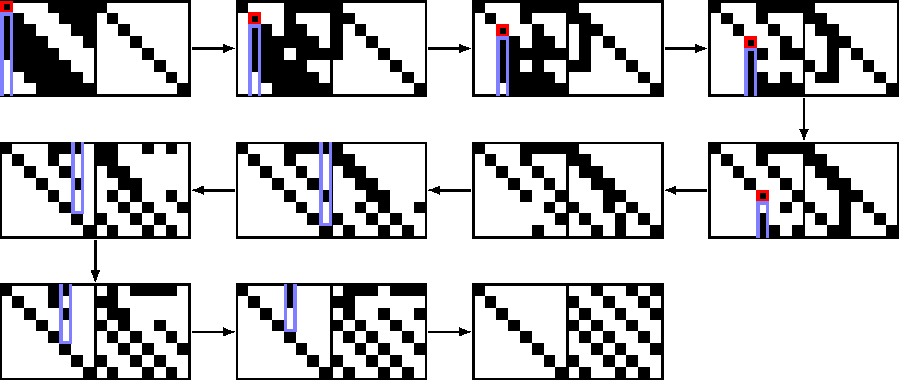
\includegraphics[width=\textwidth]{chapters/90-crypto/images/sbox.pdf}
\caption{Berechnung der Inversen der Matrix $A$ in der $S$-Box  des
AES-Algorithmus mit dem Gauss-Algorithmus
\label{buch:crypto:fig:sbox}}
\end{figure}

Eine lineare Transformation in diesem Vektorraum kann durch eine
$8\times 8$-Matrix in $M_8(\mathbb{F}_2)$ betrachtet werden.
In der $S$-Box wird die Matrix
\[
A=
\begin{pmatrix}
1&0&0&0&1&1&1&1\\
1&1&0&0&0&1&1&1\\
1&1&1&0&0&0&1&1\\
1&1&1&1&0&0&0&1\\
1&1&1&1&1&0&0&0\\
0&1&1&1&1&1&0&0\\
0&0&1&1&1&1&1&0\\
0&0&0&1&1&1&1&1
\end{pmatrix},
\qquad
A^{-1}
=
\begin{pmatrix}
0&0&1&0&0&1&0&1\\
1&0&0&1&0&0&1&0\\
0&1&0&0&1&0&0&1\\
1&0&1&0&0&1&0&0\\
0&1&0&1&0&0&1&0\\
0&0&1&0&1&0&0&1\\
1&0&0&1&0&1&0&0\\
0&1&0&0&1&0&1&0
\end{pmatrix}
\]
verwendet.
Mit dem Gauss-Algorithmus, schematisch dargestellt in
Abbildung~\ref{buch:crypto:fig:sbox}, kann man die Inverse
bestimmen, die Multiplikation mit $A$ ist also eine invertierbare
Abbildung.

Der letzte Schritt ist dann wieder eine Addition von
$q(X)=X^7+X^6+X+1\in \mathbb{F}_{2^8}$, durch Subtraktion
von $q(X)$ invertiert werden kann.
Die $S$-Box-Operation kann also bektoriell geschrieben werden also
\[
	S(x) = A\overline{x}+q.
\]

Die Implementation ist möglicherweise mit einer Tabelle am schnellsten,
es sind ja nur 256 Bytes im Definitionsbereich der $S$-Box-Abbildung
und ebenso nur 256 möglich Werte.

\subsection{Block-Operationen
\label{buch:subsection:block-operationen}}
Die zu verschlüsselnden Daten werden in in Blöcke aufgeteilt, deren
Länge Vielfache von $32$ bit sind.
Die kleinste Blockgrösse ist 128\,Bit, die grösste ist 256\,Bit.
Die Bytes eines Blockes werden dann in einem Rechteck angeordnet
als
\begin{equation}
\begin{tabular}{|>{$}c<{$}>{$}c<{$}>{$}c<{$}>{$}c<{$}>{$}c<{$}>{$}c<{$}>{$}c<{$}>{$}c<{$}|}
\hline
 b_{0} & b_{4} & b_{8}  & b_{12} & b_{16} & b_{20} & b_{24} & b_{28} \\
 b_{1} & b_{5} & b_{9}  & b_{13} & b_{17} & b_{21} & b_{25} & b_{29} \\
 b_{2} & b_{6} & b_{10} & b_{14} & b_{18} & b_{22} & b_{26} & b_{30} \\
 b_{3} & b_{7} & b_{11} & b_{15} & b_{19} & b_{23} & b_{27} & b_{31} \\
\hline
\end{tabular}
\label{buch:crypto:eqn:block}
\end{equation}
für eine Blocklänge von 256\,Bits.



\subsubsection{Zeilenshift}
\begin{figure}
\centering
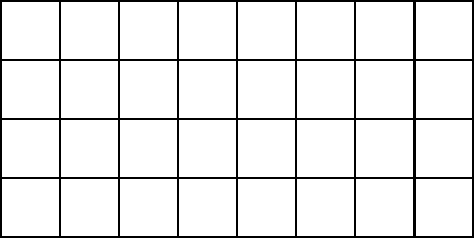
\includegraphics[width=\textwidth]{chapters/90-crypto/images/shift.pdf}
\caption{Zeilenshift in einem Block von 256 bits
\label{buch:crypto:fig:shift}}
\end{figure}
Die Verschlüsselung muss sicherstellen, dass die Bytes des Blockes
untereinander gut gemischt werden.
Die bisher beschriebenen Operationen operieren immer nur auf einzelnen
Bytes während
die im nächsten Abschnitt beschriebene Spalten-Mischoperation
nur auf Spalten wird.
Die Zeilenmischoperation permutiert die Zeilen in den vier Zeilen
eines Blocks zyklisch, die erste Zeile bleibt an Ort, die zweite
Zeile wird um ein Byte rotiert, die dritte um zwei und die letzte
um 3 Bytes, wie in Abbildung~\ref{buch:crypto:fig:zeilenshift}
dargestellt.
Diese Operation könnte mit einer Permutationsmatrix beschrieben werden,
dies wäre jedoch keine effiziente Implementation.
Der Zeilenschift hat ansonsten keine elegante algebraische Beschreibung.

\subsubsection{Spalten mischen}
Jede Spalte von \eqref{buch:crypto:eqn:block} kann als Vektor des
vierdimensionalen Vektorraumes $\mathbb{F}_{2^8}^4$.
Die Zeilenmischoperation wendet ein lineare Abbildung auf jeden
Spaltenvektor von~\eqref{buch:crypto:eqn:block}.
Die Koeffizienten der Matrix sind Elemente von $\mathbb{F}_{2^8}$.
Die Matrix ist
\[
C=\begin{pmatrix}
\texttt{02}_{16}&\texttt{03}_{16}&\texttt{01}_{16}&\texttt{01}_{16}\\
\texttt{01}_{16}&\texttt{02}_{16}&\texttt{03}_{16}&\texttt{01}_{16}\\
\texttt{01}_{16}&\texttt{01}_{16}&\texttt{02}_{16}&\texttt{03}_{16}\\
\texttt{03}_{16}&\texttt{01}_{16}&\texttt{01}_{16}&\texttt{02}_{16}
\end{pmatrix}.
\]
Um nachzuprüfen, dass die Matrix $C$ invertierbar ist, könnte man den
Gauss-Algorithmus verwenden und damit die Inverse berechnen.
Dazu müsste man die multiplikativen Inversen kennen, was etwas mühsam
ist.
Man kann aber aber auch die Determinante bestimmen, dazu braucht man
nur multiplizieren zu können, was in diesem Fall sehr leicht möglich ist,
weil kein Überlauf entsteht.
Dabei hilft es zu beachten, dass die Multiplikation mit $\texttt{02}_{16}$
nur eine Einbit-Shiftoperation nach links ist.
Nur die Multiplikation $\texttt{03}_{16}\cdot\texttt{03}_{16}=\text{05}_{16}$
gibt etwas mehr zu überlegen.
Mit geeigneten Zeilen-Operationen kann man die Berechnung der Determinante
von $C$ mit dem Entwicklungssatz etwas vereinfachen.
Man erhält
\begin{align*}
\det(C)
&=
\left|
\begin{matrix}
\texttt{02}_{16}&\texttt{03}_{16}&\texttt{01}_{16}&\texttt{01}_{16}\\
\texttt{01}_{16}&\texttt{02}_{16}&\texttt{03}_{16}&\texttt{01}_{16}\\
\texttt{00}_{16}&\texttt{03}_{16}&\texttt{01}_{16}&\texttt{02}_{16}\\
\texttt{00}_{16}&\texttt{00}_{16}&\texttt{03}_{16}&\texttt{02}_{16}
\end{matrix}
\right|
\\
&=
\texttt{02}_{16}
\left|
\begin{matrix}
\texttt{02}_{16}&\texttt{03}_{16}&\texttt{01}_{16}\\
\texttt{03}_{16}&\texttt{01}_{16}&\texttt{02}_{16}\\
\texttt{00}_{16}&\texttt{03}_{16}&\texttt{02}_{16}
\end{matrix}
\right|
+
\texttt{01}_{16}
\left|
\begin{matrix}
\texttt{03}_{16}&\texttt{01}_{16}&\texttt{01}_{16}\\
\texttt{03}_{16}&\texttt{01}_{16}&\texttt{02}_{16}\\
\texttt{00}_{16}&\texttt{03}_{16}&\texttt{02}_{16}
\end{matrix}
\right|
\\
&=
\texttt{02}_{16}
\left|
\begin{matrix}
\texttt{02}_{16}&\texttt{03}_{16}&\texttt{01}_{16}\\
\texttt{01}_{16}&\texttt{02}_{16}&\texttt{03}_{16}\\
\texttt{00}_{16}&\texttt{03}_{16}&\texttt{02}_{16}
\end{matrix}
\right|
+
\texttt{01}_{16}
\left|
\begin{matrix}
\texttt{03}_{16}&\texttt{01}_{16}&\texttt{01}_{16}\\
\texttt{00}_{16}&\texttt{00}_{16}&\texttt{01}_{16}\\
\texttt{00}_{16}&\texttt{03}_{16}&\texttt{02}_{16}
\end{matrix}
\right|
\\
&=
\texttt{02}_{16}
\left(
\texttt{02}_{16}
\left|
\begin{matrix}
\texttt{02}_{16}&\texttt{03}_{16}\\
\texttt{03}_{16}&\texttt{02}_{16}
\end{matrix}
\right|
+
\texttt{01}_{16}
\left|
\begin{matrix}
\texttt{03}_{16}&\texttt{01}_{16}\\
\texttt{03}_{16}&\texttt{02}_{16}
\end{matrix}
\right|
\right)
+
\texttt{01}_{16}
\left|
\begin{matrix}
\texttt{03}_{16}&\texttt{01}_{16}&\texttt{01}_{16}\\
\texttt{00}_{16}&\texttt{03}_{16}&\texttt{02}_{16}\\
\texttt{00}_{16}&\texttt{00}_{16}&\texttt{01}_{16}
\end{matrix}
\right|
\\
&=
\texttt{02}_{16}
(
\texttt{02}_{16}(\texttt{04}_{16}+\texttt{05}_{16})
+
(\texttt{06}_{16}+\texttt{03}_{16})
)
+
\texttt{03}_{16}\texttt{03}_{16}
\\
&=
\texttt{02}_{16}
(
\texttt{02}_{16}
+
\texttt{05}_{16}
)
+
\texttt{05}_{16}
=
\texttt{0e}_{16}+\texttt{05}_{16}
=
\texttt{0a}_{16}
\ne 0.
\end{align*}
Damit ist gezeigt, dass die Matrix $C$ invertierbar auf den
Spaltenvektoren wirkt.
Die Inverse der Matrix kann einmal berechnet und anschliessend
für die Entschlüsselung verwendet werden.

Alternativ kann man die Multiplikation mit der Matrix $C$ auch
interpretieren als eine Polynommultiplikation.
Dazu interpretiert man die Spalten des Blocks als Polynom vom Grad~3
mit Koeffizienten in $\mathbb{F}_{2^8}$.
Durch Reduktion mit dem irreduziblen Polynom
$n(Z)=Z^4+1\in\mathbb{F}_{2^8}[X]$ entsteht aus dem Polynomring
wieder ein Körper.
Die Wirkung der Matrix $C$ ist dann nichts anderes als Multiplikation
mit dem Polynom
\[
c(Z) = \texttt{03}_{16}Z^3 + Z^2+Z^1+\texttt{02}_{16},
\]
die natürlich ebenfalls umkehrbar ist.

\subsection{Schlüssel
\label{buch:subsection:schlüssel}}
Die von den Byte- und Blockoperationen mischen die einzelnen Bits
der Daten zwar ganz schön durcheinander, aber es wird noch kein
Schlüsselmaterial eingearbeitet, welches den Prozess einzigartig
macht.

\subsubsection{Schlüsseladdition}
Nach jeder Spaltenmischoperation wird ein Rundenschlüssel
zum Blockhinzuaddiert.
Beim ersten Mal wird dazu einfach das Schlüsselmaterial verwendet.
Für die folgenden Runden muss aus diesem Schlüssel neues
Material, die sogenannten Rundenschlüssel, gewonnen werden.

\subsubsection{Rundenschlüssel}
\begin{figure}
\centering
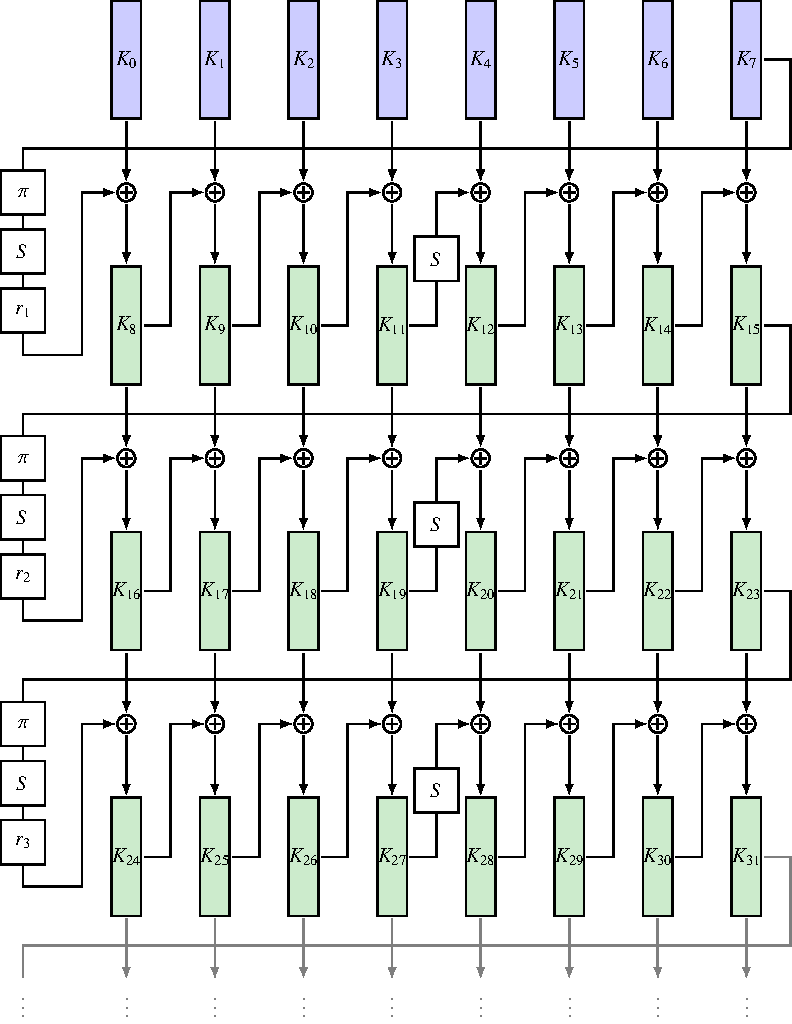
\includegraphics{chapters/90-crypto/images/keys.pdf}
\caption{Erzeugung der erweiterten Schlüsseldaten aus dem Schlüssel
$K_0,\dots,K_7$ für Schlüssellänge 256\,bit.
Die mit $S$ beschrifteten Blöcke wenden die $S$-Box auf jedes einzelne
Byte an.
$\pi$ ist die zyklische Vertauschung der Bytes eines Wortes.
Die Operation $r_i$ ist eine Addition einer Konstanten, die in jeder
Runde anders ist.
\label{buch:crypto:fig:keys}}
\end{figure}
Die Erzeugung der Rundenschlüssel ist in Abbildung
\ref{buch:crypto:fig:keys}
schematisch dargestellt.
Die Blöcke beschreiben wieder Spaltenvektoren im vierdimensionalen
Raum $\mathbb{F}_{2^8}^4$.
Die Blöcke $K_0$ bis $K_7$ stellen den ursprünglichen Schlüssel dar.
Die Erzeugung eines neuen Blocks Schlüsselmatrial beginnt damit,
dass der letzte Vektor des vorangegangenblocks drei Operationen
unterworfen werden.
\begin{itemize}
\item
Die Operation $\pi$ vertauscht die Bytes des Vektors zyklisch:
\begin{center}
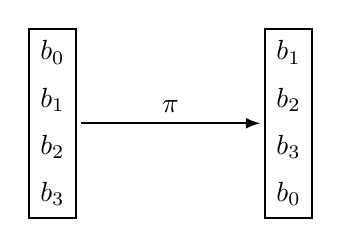
\begin{tikzpicture}[>=latex,thick]
\def\s{0.6}
\begin{scope}
\draw (0,0) rectangle (\s,{4*\s});
\foreach \y in {1,...,3}{
	\draw (0,{\y*\s}) (\s,{\y*\s});
}
\node at ({0.5*\s},{0.5*\s}) {$b_3$};
\node at ({0.5*\s},{1.5*\s}) {$b_2$};
\node at ({0.5*\s},{2.5*\s}) {$b_1$};
\node at ({0.5*\s},{3.5*\s}) {$b_0$};
\end{scope}
\draw[->] ({1.1*\s},{2*\s}) -- ({4.9*\s},{2*\s});
\node at ({3*\s},{2*\s}) [above] {$\pi$};
\begin{scope}[xshift=3cm]
\draw (0,0) rectangle (\s,{4*\s});
\foreach \y in {1,...,3}{
	\draw (0,{\y*\s}) (\s,{\y*\s});
}
\node at ({0.5*\s},{0.5*\s}) {$b_0$};
\node at ({0.5*\s},{1.5*\s}) {$b_3$};
\node at ({0.5*\s},{2.5*\s}) {$b_2$};
\node at ({0.5*\s},{3.5*\s}) {$b_1$};
\end{scope}
\end{tikzpicture}
\end{center}
\item
Die $S$-Operation wendet die $S$-Box auf alle Bytes eines Vektors an.
\item
Die $r_i$ Operation addiert in Runde eine Konstante $r_i$ zur $0$-Komponente.
\end{itemize}
Die Konstante $r_i$ ist wieder ein einzelnes Byte und es ist daher
naheliegend, diese Bytes mit Hilfe der Arithmetik in $\mathbb{F}_{2^8}$
zu erzeugen.
Man kann daher $r_i$ definieren als
$(\texttt{02}_{16})^{i-1}\in\mathbb{F}_{2^8}$.

\subsection{Runden}
Der AES-Verschlüsselungsalgorithmus besteht jetzt darin, die bisher
definierten Operationen wiederholt anzuwenden.
Eine einzelne Runde besteht dabei aus folgenden Schritten:
\begin{enumerate}
\item Wende die $S$-Box auf alle Bytes des Blocks an.
\item Führe den Zeilenshift durch.
\item Mische die Spalten (wird in der letzten Runde)
\item Erzeuge den nächsten Rundenschlüssel
\item Addiere den Rundenschlüssel
\end{enumerate}
Der AES-Verschlüsselungsalgorithmus beginnt damit, dass der Schlüssel
zum Datenblock addiert wird.
Anschliessend werden je nach Blocklänge verschiedene Anzahlen von
Runden durchgeführt, 10 Runden für 128\,bit, 12 Runden für 192\,bit und
14 Runden für 256\,bit.





